
\documentclass{beamer}
\usepackage{multicol}

\usepackage{tikz}
\usepackage{ifthen}
\usepackage{xstring}
\usepackage{calc}
\usepackage{pgfopts}
\usepackage{tikz-uml}
\usetikzlibrary{shapes.geometric, arrows}

\tikzstyle{startstop} = [rectangle, rounded corners, minimum width=3cm, minimum height=1cm,text centered, draw=black, fill=red!30]
\tikzstyle{process} = [rectangle, minimum width=2cm, minimum height=.5cm, text centered, draw=black, fill=orange!10]
\tikzstyle{arrow} = [thick,->,>=stealth] % ,>=stealth

\usepackage{tikz-timing}
\usetikztiminglibrary[new={char=Q,reset char=R}]{counters}

\usepackage{graphicx}
\DeclareGraphicsExtensions{.pdf,.png,.jpg}




\begin{document}
\title{Group 9 \\
	   ECSE 426}   
\author{Matthew Vertescher \\ 
		Christopher Mcgirr \\
		Pandit Adhilaga-Dres} 
\date{\today} 

\frame{\titlepage} 

%\frame{\frametitle{Table of contents}\tableofcontents} 
\frame{\frametitle{Table of contents} 
\begin{multicols}{2}
  \tableofcontents
\end{multicols}
}

\section{Wireless Design} 
\frame{\frametitle{Wireless Design Overview} 
	Major components:	
	\begin{itemize}
		\item CC2500 SPI Driver 
		\item Wireless broadcast and listener
		\item Pitch, roll, time protocol 
		\item Recorded sequence protocol 
		\item Signal strength LED 
	\end{itemize} 
}

\subsection{CC2500 SPI}
\frame{\frametitle{CC2500 SPI} 
	\begin{itemize}
		\item Connection to eZ430-RF2500 target board forwards pins to CC2500 
		\item SPI linked via four wires
		\begin{itemize}
			\item SCK 	:	SPI Clock, 6.5MHz
			\item MOSI 	: 	Master out, slave in
			\item MISO 	: 	Master in, slave out
			\item CS 	: 	Chip select 
		\end{itemize} 
		\item Header Byte
		\begin{itemize}
			\item Bit 7		 : Read / Write  
			\item Bit 6		 : Burst mode
			\item Bits [5:0] : Register address 
		\end{itemize} 
		\item Data byte(s)
	\end{itemize} 
}

\subsubsection{Reads and Writes}
\frame{\frametitle{Reads and Writes} 
\begin{center}
\begin{tikztimingtable}
  [timing/d/background/.style={fill=white},
   timing/lslope=0.2,scale=1.1]
 		  SCK 	 & LLL 15{T} LLL \\    % CPOL = 0             
          CS     & H 19L L     \\
		  MOSI & LL 2D{R/W} 2D{B} 2D{A$_5$} 2D{A$_4$} 2D{A$_3$} 2D{A$_2$} 2D{A$_1$} 2D{A$_0$} LLL \\           
          MISO & LL 2D{RDY} 2D{S$_3$} 2D{S$_2$} 2D{S$_1$} 2D{F$_3$} 2D{F$_2$} 2D{F$_1$} 2D{F$_0$} LLL \\ 
            \\
          CS     & L 19L H     \\
	 	  MOSI & LL 2D{W$_7$} 2D{W$_6$} 2D{W$_5$} 2D{W$_4$} 2D{W$_3$} 2D{W$_2$} 2D{W$_1$} 2D{W$_0$} LLL \\  
	 	  MISO & LL 2D{RDY} 2D{S$_3$} 2D{S$_2$} 2D{S$_1$} 2D{F$_3$} 2D{F$_2$} 2D{F$_1$} 2D{F$_0$} LLL \\ 
	 	  \\ 
	 	  MOSI & L 19L L \\         
          MISO & LL 2D{R$_7$} 2D{R$_6$} 2D{R$_5$} 2D{R$_4$} 2D{R$_3$} 2D{R$_2$} 2D{R$_1$} 2D{R$_0$} LLL \\      
\extracode
  % Add vertical lines in two colors
  \begin{pgfonlayer}{background}
    \begin{scope}[semitransparent,semithick]
      \vertlines[blue]{2.1,4.1,...,18.1}
      \vertlines[red]{3.1,5.1,...,17.1}
    \end{scope}
  \end{pgfonlayer}
  % Add big group labels
  \begin{scope}
    [font=\sffamily\Large,shift={(-4em,-0.5)},anchor=east]
    %\node at (  0, 0) {SCK};    \node at (  0,-3 ) {SS};
    \node at (1ex,-12) {R/W = 0}; \node at (1ex,-18) {R/W = 1};
  \end{scope}
\end{tikztimingtable}%
\end{center}
}

\subsubsection{Command Strobes}
\frame{\frametitle{Command Strobes} 
\begin{center}
\begin{tikztimingtable}
  [timing/d/background/.style={fill=white},
   timing/lslope=0.2,scale=1.6]
          CS     & H 19L H     \\
          SCK 	 & LLL 15{T} LLL \\    % CPOL = 0   
        %Cycle \# & U     R 2D{Text} 2U    \\ %8{2Q}
			MOSI & LL 2D{R/W} 2D{B} 2D{A$_5$} 2D{A$_4$} 2D{A$_3$} 2D{A$_2$} 2D{A$_1$} 2D{A$_0$} LLL \\           
            MISO & LL 2D{RDY} 2D{S$_3$} 2D{S$_2$} 2D{S$_1$} 2D{F$_3$} 2D{F$_2$} 2D{F$_1$} 2D{F$_0$} LLL \\ 
\extracode
  % Add vertical lines in two colors
  \begin{pgfonlayer}{background}
    \begin{scope}[semitransparent,semithick]
      \vertlines[blue]{2.1,4.1,...,18.1}
      \vertlines[red]{3.1,5.1,...,17.1}
    \end{scope}
  \end{pgfonlayer}
  % Add big group labels
  %\begin{scope}
  %  [font=\sffamily\Large,shift={(-6em,-0.5)},anchor=east]
  %  \node at (  0, 0) {SCK};    \node at (  0,-3 ) {SS};
  %  \node at (1ex,-9) {CPHA=0}; \node at (1ex,-17) {CPHA=1};
  %\end{scope}
\end{tikztimingtable}%
\end{center}
}

\subsubsection{FIFO Buffers}
\frame{\frametitle{FIFO Buffers} 
	\begin{itemize}
		\item Two 64B FIFO Buffers RX and TX
		\item To transmit: place data into FIFO buffer and move to TX state
		\item To receive: read from RX FIFO 
		\item Single address, access determined by R/W and B bits of the SPI header 
	\end{itemize} 
}

\subsection{Packet Description}
\frame{\frametitle{Fixed Packet} 
	\begin{itemize}
		\item $f_{carrier} = 2.4347 GHz$
		\item Fixed packet length of 10 bytes
		\item Two floats used for pitch, roll and time
		\item CTRL1 : data command byte 
		\item CTRL2 : counter utility byte
	\end{itemize} 	
	\begin{center}
	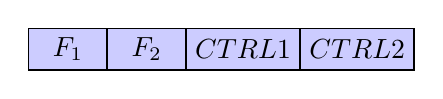
\begin{tikzpicture}[>=latex,font=\sffamily,every node/.style={minimum width=1cm,minimum 				height=1.5em,outer sep=0pt,draw=black,fill=blue!20,semithick}]
        \node at (0,0) (A) {$F_1$};
        \node [anchor=west] at (A.east) (B) {$F_2$};
        \node [anchor=west] at (B.east) (C) {$CTRL1$};
        \node [anchor=west] at (C.east) (D) {$CTRL2$};
        %\draw [->,shorten >=2pt,shorten <=2pt,semithick] (G.south) -- +(0,-1em) -| (A);
	\end{tikzpicture}
	\end{center}
}

%\subsection{Core Functionality}
%\frame{\frametitle{Core Functionality} 
%	\begin{itemize}
%		\item 
%	\end{itemize}
%}


\subsection{Acceleration Broadcast}
\frame{\frametitle{Acceleration Broadcast} 
\begin{multicols}{2}	
	\begin{center}	
	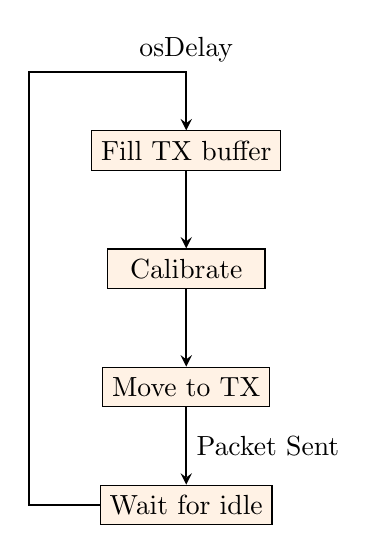
\begin{tikzpicture}[node distance=1.5cm]

	%\node (start) [startstop] {Start};
	\node (tx) [process] {Fill TX buffer};
	\node (cal) [process, below of=tx] {Calibrate};
	\node (send) [process, below of=cal] {Move to TX};
	\node (idle) [process, below of=send] {Wait for idle};
	
	\draw [arrow] (tx) -- node[anchor=east] {} (cal);
	\draw [arrow] (cal) -- node[anchor=east] {} (send);
	\draw [arrow] (send) -- node[anchor=west] {Packet Sent} (idle);
	\draw [arrow] (idle) -- ++(-2,0) -- ++(0,5.5) -|  node[anchor=south] {osDelay} (tx);
	
	\end{tikzpicture}
	\end{center}	
	
	\begin{center}	
	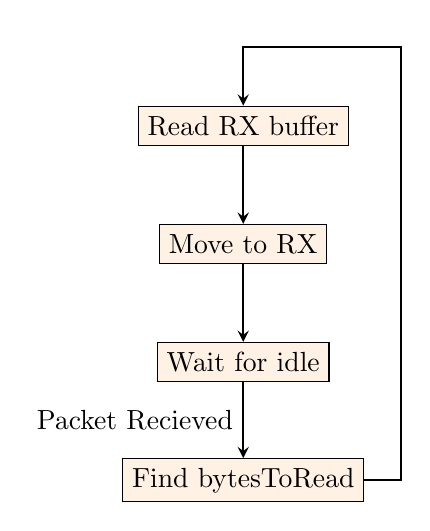
\begin{tikzpicture}[node distance=1.5cm]

	%\node (start) [startstop] {Start};
	\node (tx) [process] {Read RX buffer};
	\node (cal) [process, below of=tx] {Move to RX};
	\node (send) [process, below of=cal] {Wait for idle};
	\node (idle) [process, below of=send] {Find bytesToRead};
	
	\draw [arrow] (tx) -- node[anchor=east] {} (cal);
	\draw [arrow] (cal) -- node[anchor=east] {} (send);
	\draw [arrow] (send) -- node[anchor=east] {Packet Recieved} (idle);
	\draw [arrow] (idle) -- ++(2,0) -- ++(0,5.5) -|  node[anchor=south] {} (tx);
	
	\end{tikzpicture}
	\end{center}	
\end{multicols}
%	\begin{center}
%	
% 	\begin{tikzpicture} 
%	\begin{umlstate}[name=tran, fill=blue!10]{Transmitter} 
%	\begin{umlstate}[name=tx, fill=red!20]{Fill TX buffer}\end{umlstate} 
%	\begin{umlstate}[x=0, y=-3, name=cal, fill=red!20]{Calibrate}\end{umlstate} 
%	\begin{umlstate}[x=5, y=-3, name=send, fill=red!20]{TX Sending}\end{umlstate} 	
%	\begin{umlstate}[x=5, y=0, name=idle, fill=red!20]{Wait for idle}\end{umlstate} 		
%		
%	\umltrans{tx}{cal} 
%	\umltrans{cal}{send} 
%	\umltrans{send}{idle} 
%	\umltrans{idle}{tx} 
%	%\begin{umlstate}[x=3, y=-3, name=substate2]{I am a substate 2} 
%
%	\end{umlstate} 	
%	\end{tikzpicture}
%	\end{center}
}


\subsection{Pitch Roll Time Protocol}
\frame{\frametitle{Pitch Roll Time Protocol} 
	\begin{enumerate}
		\item On button press, the transmitter stops broadcasting pitch and roll.
		\item The transmitter then sends a control packet to the receiver informing it to process the following packets as pitch, roll and time.  
		\item The transmitter listens for the pitch, roll and time to all be updated.
		\begin{enumerate}
			\item Packets are sent from the transmitter to receiver containing the pitch, roll and time.
		\end{enumerate}				
		\item A final control packet is send to indicated to the receiver to execute the programmed sequence.
		\item After a sufficient delay the transmitter return to broadcast mode.
	\end{enumerate}
}

\subsection{Record and Play Protocol}
\frame{\frametitle{Record and Play Protocol} 
	\begin{enumerate}
		\item On button press, the transmitter stops broadcasting pitch and roll.
		\item The transmitter then begins recording 256 accelerometer data samples at 10Hz.
		\item Once the recoding has finished, the transmitter sends a start control packet, 256 data packets, and an end control packet. 
		\item After the ending control packet is processed, the receiver plays back the sequence.
		\begin{enumerate}
			\item To reconstruct the sequence, the receiver interpolates the data back to 100Hz in real time.
		\end{enumerate}				
		
	\end{enumerate}
}

\subsection{Signal Strength LED}
\frame{\frametitle{Signal Strength LED} 
	\begin{itemize}
		\item By reading the RSSI, received signal strength indicator, DB signal strength value can be calculated for the current channel.
		\item RSSI value is updated in the RX state.
		\item In broadcast mode, the RSSI value is read every time a packet is read. 
		\item PWM and a LED are used to indicate the power.
	\end{itemize}
}


\section{Mechanical and System Design} 
\frame{\frametitle{System Design Overview}
	\begin{itemize}
		\item Keyboard and state machine  
		\item Servo motor system
		\item Feedback
	\end{itemize} 
}

\subsection{Keyboard State Machine} 
\frame{\frametitle{Keyboard State Machine}
	
	\begin{center}
		\includegraphics[width=10cm]{./images/KeyboardStateDiagram}
	\end{center}
	
}

\subsection{Servo Motor System} 
\frame{\frametitle{Servo Motor System}
	\begin{multicols}{2}
		\begin{center}
			\includegraphics[width=5cm]{./images/MechDesignTopNewPage}
		\end{center}
		\begin{center}
			\includegraphics[width=5cm]{./images/MechDesignMechDesignSide}
		\end{center}
	\end{multicols}
}

\subsection{Feedback}
\frame{\frametitle{Feedback} 
	\begin{itemize}
		\item The servo motor system can get feedback from the receiver's accelerometer.
		\item The system attempts to converge the pitch and roll measured on the receiver to the desired pitch and roll sent from the transmitter.
		\item This system attempts to correct servo motor error.
	\end{itemize}
}



\section{Integration and Testing}
\subsection{Module Overview}
\frame{\frametitle{Module Overview}
	\begin{center}
	
 	\begin{tikzpicture} 
	%\begin{umlstate}[name=tran, fill=blue!10]{Transmitter} 
	\begin{umlstate}[name=main, fill=yellow!20]{Main}\end{umlstate} 
	\begin{umlstate}[x=0, y=-3, name=A, fill=yellow!20]{Auxiliary Files}\end{umlstate} 
	\begin{umlstate}[x=5, y=0, name=B, fill=yellow!20]{Application Drivers}\end{umlstate} 	
	\begin{umlstate}[x=5, y=-3, name=C, fill=yellow!20]{General Drivers}\end{umlstate} 		
		
	\umltrans{A}{main} 
	\umltrans{B}{main} 
	\umltrans{C}{B} 
	%\umltrans{idle}{tx} 
	%\begin{umlstate}[x=3, y=-3, name=substate2]{I am a substate 2} 

	%\end{umlstate} 	
	\end{tikzpicture}
	\end{center}
}

\subsection{Transmitter Event Diagram}
\frame{\frametitle{Transmitter Event Diagram}
	\begin{center}
			\includegraphics[width=10cm]{./images/transmitter_events}
		\end{center}
}

\subsection{Receiver Event Diagram}
\frame{\frametitle{Receiver Event Diagram}	
	\begin{center}
			\includegraphics[width=10cm]{./images/receiver_events}
	\end{center}
}

\subsection{Challenges}
\frame{\frametitle{Challenges}
	\begin{itemize}
		\item Packet noise during development 
		\item Achieving reliable transmissions without handshakes
		\item Feedback system 
		\item Signal strength 
	\end{itemize}
}



%\section{Section no. 2} 
%\subsection{Lists I}
%\frame{\frametitle{unnumbered lists}
%\begin{itemize}
%\item Introduction to  \LaTeX  
%\item Course 2 
%\item Termpapers and presentations with \LaTeX 
%\item Beamer class
%\end{itemize} 
%}
%
%\frame{\frametitle{lists with pause}
%\begin{itemize}
%\item Introduction to  \LaTeX \pause 
%\item Course 2 \pause 
%\item Termpapers and presentations with \LaTeX \pause 
%\item Beamer class
%\end{itemize} 
%}
%
%\subsection{Lists II}
%\frame{\frametitle{numbered lists}
%\begin{enumerate}
%\item Introduction to  \LaTeX  
%\item Course 2 
%\item Termpapers and presentations with \LaTeX 
%\item Beamer class
%\end{enumerate}
%}
%\frame{\frametitle{numbered lists with pause}
%\begin{enumerate}
%\item Introduction to  \LaTeX \pause 
%\item Course 2 \pause 
%\item Termpapers and presentations with \LaTeX \pause 
%\item Beamer class
%\end{enumerate}
%}
%
%\section{Section no.3} 
%\subsection{Tables}
%\frame{\frametitle{Tables}
%\begin{tabular}{|c|c|c|}
%\hline
%\textbf{Date} & \textbf{Instructor} & \textbf{Title} \\
%\hline
%WS 04/05 & Sascha Frank & First steps with  \LaTeX  \\
%\hline
%SS 05 & Sascha Frank & \LaTeX \ Course serial \\
%\hline
%\end{tabular}}
%
%
%\frame{\frametitle{Tables with pause}
%\begin{tabular}{c c c}
%A & B & C \\ 
%\pause 
%1 & 2 & 3 \\  
%\pause 
%A & B & C \\ 
%\end{tabular} }
%
%
%\section{Section no. 4}
%\subsection{blocs}
%\frame{\frametitle{blocs}
%
%\begin{block}{title of the bloc}
%bloc text
%\end{block}
%
%\begin{exampleblock}{title of the bloc}
%bloc text
%\end{exampleblock}
%
%
%\begin{alertblock}{title of the bloc}
%bloc text
%\end{alertblock}
%}


\end{document}
